% Generated from data/synthetic_evaluation/evaluation.json. Do not edit numbers manually.
\subsection{Phân tích chỉ số trên bộ số liệu tổng hợp}
\subsubsection{Nguồn gốc và cấu trúc dữ liệu}
\label{sec:synthetic-origin}
Bộ dữ liệu trong phần này được tạo bằng chương trình với hạt giống ngẫu nhiên cố định 20260917. Dữ liệu gồm số đếm phân loại và các bản ghi thời lượng, không phải video đã chạy qua mô hình thị giác máy tính. Các tham số được chọn để bao phủ ca làm có độ dài khác nhau, trường hợp dưới và trên hạn mức điện thoại, khoảng mất quan sát và một số sai số lớn. Đây là các giả định thiết kế chưa được hiệu chỉnh theo dữ liệu thực địa.

Các bảng dưới đây được tính lại từ cùng tệp dữ liệu nguồn. Mã SYN-P và SYN-C nhận diện bản ghi tổng hợp. Các giá trị hiển thị được làm tròn đến số chữ số đã công bố, với trường hợp đúng nửa đơn vị làm tròn lên về độ lớn. Chỉ số tổng hợp được tính từ dữ liệu chưa làm tròn.

Năm khối dữ liệu độc lập gồm số đếm phát hiện người, số đếm hiện diện, số đếm sử dụng điện thoại, 12 phiên điện thoại và 30 ca. Không ghép các khối này thành một tập quan sát chung hoặc suy ra quan hệ nhân quả giữa chúng. Ba mức S1, S2 và S3 biểu diễn mức nhiễu tăng dần, không đại diện ba thuật toán đã được chạy.

\begin{table}[H]
\centering
\caption{Các giả định của bộ dữ liệu tổng hợp}
\label{tab:synthetic-assumptions}
\begin{tabularx}{\textwidth}{p{4.4cm}X}
\toprule
Thành phần & Quy tắc tạo dữ liệu\\
\midrule
Thời lượng ca & 4, 6 hoặc 8 giờ\\
Mất quan sát & 0, 30, 90 hoặc 180 giây, lưu riêng với vắng mặt\\
Hiện diện tham chiếu & 76--96\% thời gian có quan sát\\
Điện thoại trong ca & 0--2700 giây, có mẫu tại ngưỡng hạn mức\\
Hạn mức điện thoại & 900 giây mỗi ca, dùng để kiểm tra công thức\\
Nhiễu thời lượng hiện diện & Phân phối chuẩn với trung bình $-35$ giây, độ lệch chuẩn 65 giây\\
Nhiễu thời lượng điện thoại & Phân phối chuẩn với trung bình $-5$ giây, độ lệch chuẩn 25 giây\\
Trường hợp sai số lớn & Ca 10, 20 và 30 thêm sai lệch có độ lớn 180--330 giây\\
Mức nhiễu S1/S2/S3 & Nhân cùng sai lệch cơ sở lần lượt với 1, 2 và 4\\
\bottomrule
\end{tabularx}
\end{table}

Thời lượng được làm tròn đến giây và giới hạn trong miền hợp lệ. Thời gian điện thoại không vượt thời gian hiện diện, thời gian hiện diện không vượt thời gian có quan sát. Các ràng buộc này bảo đảm tính nhất quán số học, nhưng không xác nhận rằng phân phối nhiễu phản ánh một camera hoặc một mô hình cụ thể.

\subsubsection{Kiểm tra chỉ số phát hiện người bằng số đếm tổng hợp}
Đơn vị tham chiếu là một đối tượng người tại một thời điểm quan sát, không phải một khung hình. Bảng sử dụng 10.000 đối tượng tham chiếu. TP, FP và FN là số đếm được khai báo trong bộ tổng hợp để kiểm tra công thức Precision, Recall và F1. Tổng hợp được tính từ tổng số đếm, không lấy trung bình các tỉ lệ theo số khung hình.
\begin{table}[H]
\centering
\small
\caption{Chỉ số phát hiện người từ số đếm tổng hợp}
\label{tab:syn-person}
\begin{tabular}{lrrrrrr}
\toprule
Điều kiện & TP & FP & FN & P & R & F1\\
\midrule
Ít che khuất & 3063 & 91 & 137 & 0,971 & 0,957 & 0,964\\
Che khuất nhẹ & 2539 & 139 & 261 & 0,948 & 0,907 & 0,927\\
Che khuất vừa & 1987 & 184 & 413 & 0,915 & 0,828 & 0,869\\
Sát biên vùng & 1271 & 152 & 329 & 0,893 & 0,794 & 0,841\\
Tổng & 8860 & 566 & 1140 & 0,940 & 0,886 & 0,912\\
\bottomrule
\end{tabular}
\end{table}
Tên điều kiện và số đếm được khai báo để minh họa cách phân nhóm. Chỉ số ở hàng tổng được tính theo tổng TP, FP, FN, nhờ đó tránh sai lệch do lấy trung bình không trọng số giữa các nhóm có quy mô khác nhau.

\subsubsection{Kiểm tra chỉ số hiện diện trên cùng tập tham chiếu}
Mỗi kịch bản có 36.000 mẫu người--giây, trong đó 27.000 mẫu hiện diện và 9.000 mẫu vắng mặt. Khoảng mất quan sát không nằm trong tập phân loại này. Vì mỗi mẫu có độ dài một giây, FN chính là số giây vắng mặt giả và FP chính là số giây hiện diện giả.
\begin{table}[H]
\centering
\small
\caption{Chỉ số hiện diện trên ba kịch bản nhiễu tổng hợp}
\label{tab:syn-presence}
\begin{tabular}{lrrrrrrr}
\toprule
Mức & TP & FP (s) & FN (s) & TN & P & R & F1\\
\midrule
S1 & 26190 & 430 & 810 & 8570 & 0,984 & 0,970 & 0,977\\
S2 & 25110 & 810 & 1890 & 8190 & 0,969 & 0,930 & 0,949\\
S3 & 23490 & 1440 & 3510 & 7560 & 0,942 & 0,870 & 0,905\\
\bottomrule
\end{tabular}
\end{table}
\begin{figure}[H]
\centering
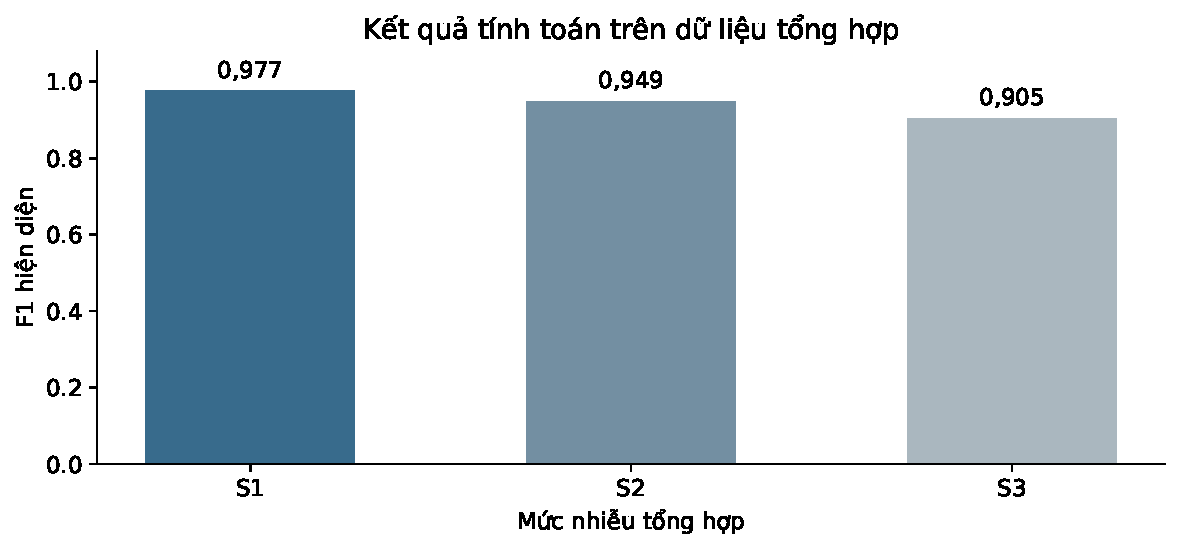
\includegraphics[width=0.88\textwidth]{Images/synthetic_presence_f1.pdf}
\caption{F1 hiện diện tính từ số đếm tổng hợp}
\label{fig:synthetic-presence}
\end{figure}
Ba hàng có cùng số mẫu dương và âm, nên thay đổi Recall có thể đối chiếu trực tiếp với số giây vắng mặt giả. F1 giảm khi tăng các số đếm lỗi theo giả định. S1, S2 và S3 không tương ứng với các cấu hình thuật toán trong quy trình đánh giá video.

\subsubsection{Kiểm tra chỉ số sử dụng và liên kết điện thoại}
Mỗi điều kiện có 3.000 mẫu người--giây. Bốn điều kiện đầu có 1.000 mẫu sử dụng và 2.000 mẫu không sử dụng. Điều kiện chỉ đặt điện thoại trên bàn có toàn bộ 3.000 mẫu âm, do đó Recall và F1 không được báo cáo. Tỉ lệ dương tính giả được tính theo $FPR=FP/(FP+TN)$.
\begin{table}[H]
\centering
\small
\caption{Phân loại sử dụng điện thoại từ số đếm tổng hợp}
\label{tab:syn-phone}
\begin{tabular}{lrrrrrrr}
\toprule
Điều kiện & TP & FP & FN & P & R & F1 & FPR\\
\midrule
Một người & 920 & 73 & 80 & 0,926 & 0,920 & 0,923 & 0,037\\
Nhiều người & 845 & 110 & 155 & 0,885 & 0,845 & 0,864 & 0,055\\
Che khuất tay & 728 & 132 & 272 & 0,847 & 0,728 & 0,783 & 0,066\\
Gần hai người & 760 & 148 & 240 & 0,837 & 0,760 & 0,797 & 0,074\\
Chỉ đặt trên bàn & 0 & 64 & 0 & 0,000 & -- & -- & 0,021\\
\bottomrule
\end{tabular}
\end{table}
WPAR sử dụng đơn vị sự kiện đã được gán người, khác với đơn vị người--giây của bảng phân loại. Các số đếm sự kiện bên dưới là một khối giả định riêng, không được dùng thay mẫu số của Precision hoặc Recall. Trường hợp không có sự kiện được gán có WPAR không xác định, ký hiệu bằng dấu gạch ngang.
\begin{table}[H]
\centering
\small
\caption{Sai gán người trên các sự kiện điện thoại tổng hợp}
\label{tab:syn-owner}
\begin{tabular}{lrrr}
\toprule
Điều kiện & Đã gán & Gán sai & WPAR\\
\midrule
Một người & 80 & 1 & 0,013\\
Nhiều người & 110 & 4 & 0,036\\
Che khuất tay & 95 & 6 & 0,063\\
Gần hai người & 105 & 9 & 0,086\\
Chỉ đặt trên bàn & 0 & 0 & --\\
\bottomrule
\end{tabular}
\end{table}
\subsubsection{Sai số thời lượng của 12 phiên điện thoại tổng hợp}
Thời lượng tham chiếu của 12 phiên được khai báo trong dữ liệu nguồn. Sai lệch được lấy từ phân phối chuẩn có trung bình $-2$ giây và độ lệch chuẩn $6+0{,}035T$ giây, với $T$ là thời lượng tham chiếu. Các giả định này tạo cả sai số tăng và giảm thời lượng, chưa mô tả sai số đo được của mô hình.
\begin{table}[H]
\centering
\small
\caption{Toàn bộ 12 phiên điện thoại tổng hợp, đơn vị giây}
\label{tab:syn-phone-duration}
\begin{tabular}{lrrr}
\toprule
Mã phiên & Tham chiếu & Ước lượng tổng hợp & Sai số có dấu\\
\midrule
SYN-P01 & 34 & 24 & -10\\
SYN-P02 & 49 & 39 & -10\\
SYN-P03 & 76 & 92 & +16\\
SYN-P04 & 123 & 118 & -5\\
SYN-P05 & 188 & 185 & -3\\
SYN-P06 & 247 & 256 & +9\\
SYN-P07 & 326 & 334 & +8\\
SYN-P08 & 418 & 432 & +14\\
SYN-P09 & 507 & 482 & -25\\
SYN-P10 & 633 & 681 & +48\\
SYN-P11 & 746 & 764 & +18\\
SYN-P12 & 858 & 846 & -12\\
\bottomrule
\end{tabular}
\end{table}
MAE tính trên toàn bộ 12 phiên là 14,83 giây/phiên, trung vị sai số tuyệt đối là 11,00 giây và sai số tuyệt đối lớn nhất là 48 giây. Các giá trị này có thể tính lại trực tiếp từ bảng, không suy ra từ một tập mẫu chưa công bố.

\subsubsection{Sai số thời gian hiệu lực trên 30 ca tổng hợp}
Mỗi ca có thời lượng hiện diện và điện thoại tham chiếu. Sau khi bổ sung nhiễu, chương trình tính lại phần vượt hạn mức và thời gian hiệu lực cho từng mức S1, S2, S3 bằng cùng công thức ở Chương 1. Sai số được tính trên thời gian hiệu lực của cùng một ca. Khoảng mất quan sát được báo riêng, không tự động cộng vào hiện diện hoặc diễn giải là vắng mặt.
\begin{table}[H]
\centering
\small
\caption{Sai số thời gian hiệu lực trên 30 ca tổng hợp}
\label{tab:syn-worktime}
\begin{tabular}{lrrrrr}
\toprule
Mức & MAE (s/ca) & MAPE (\%) & Trung vị (s) & P95 (s) & Max (s)\\
\midrule
S1 & 73,40 & 0,44 & 42,50 & 253,50 & 306\\
S2 & 146,93 & 0,87 & 85,00 & 507,10 & 612\\
S3 & 295,80 & 1,76 & 169,00 & 1028,60 & 1224\\
\bottomrule
\end{tabular}
\end{table}
P95 sử dụng nội suy tuyến tính tại vị trí $(N-1)\times0{,}95$ trong dãy sai số tuyệt đối đã sắp tăng dần. MAPE chỉ tính trên thời lượng tham chiếu dương. Trong bộ này, cả 30 ca đều đáp ứng điều kiện. Các mức nhiễu sử dụng chung sai lệch cơ sở, vì vậy không được xem là các lần thử độc lập để kiểm định ưu thế thuật toán.
\begin{figure}[H]
\centering
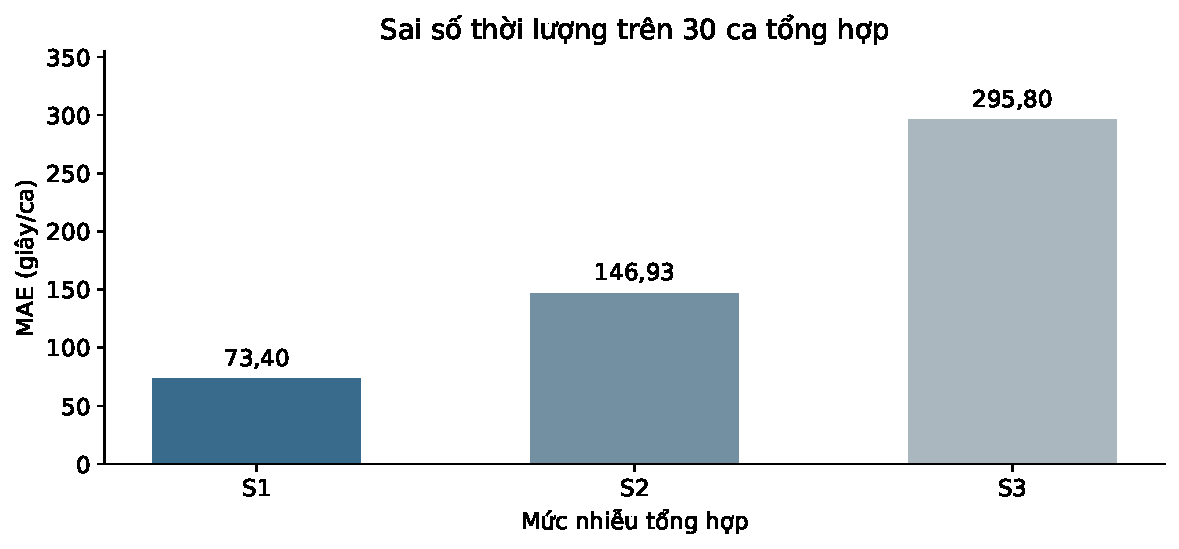
\includegraphics[width=0.88\textwidth]{Images/synthetic_time_mae.pdf}
\caption{MAE thời gian hiệu lực theo mức nhiễu tổng hợp}
\label{fig:synthetic-mae}
\end{figure}
\begin{figure}[H]
\centering
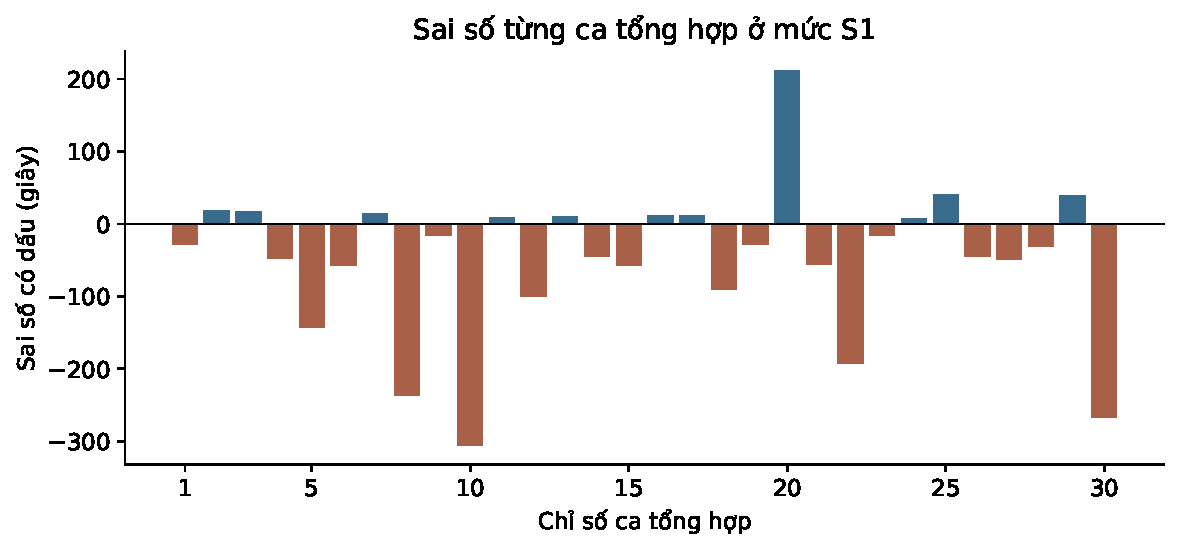
\includegraphics[width=0.88\textwidth]{Images/synthetic_shift_errors.pdf}
\caption{Sai số có dấu của 30 ca tổng hợp ở mức S1}
\label{fig:synthetic-errors}
\end{figure}
Phụ lục E công bố đủ 30 ca ở mức S1. Tệp dữ liệu nguồn lưu cả ba mức nhiễu cùng thời gian điện thoại trước và sau nhiễu. Mẫu không sử dụng điện thoại, mẫu đúng hạn mức và mẫu vừa vượt hạn mức giúp kiểm tra tính liên tục của phép điều chỉnh thời gian. Khối dữ liệu này chỉ chứa tổng thời lượng, không có mốc phiên để phân tích sai số biên. Kiểm thử phép xử lý khoảng được trình bày riêng tại mục~\ref{sec:interval-evaluation}.

\subsubsection{Lưu trữ và tái tạo số liệu}
Tệp \path{data/synthetic_evaluation/evaluation.json} lưu toàn bộ số đếm, thời lượng và chỉ số. Bản kê đi kèm công bố hạt giống, giả định, quy mô và mã SHA-256. Bộ dữ liệu giữ nguyên 12 phiên và 30 ca đã có, các giá trị không được thay đổi để tạo mức sai số thuận lợi hơn. Chạy \texttt{python generate\_synthetic\_evaluation.py} để tạo lại các bảng và hình.

